

%\chapter{An Experimental Program in Neutrinos, Nucleon Decay and Astroparticle Physics Enabled by the Fermilab Long-Baseline Neutrino Facility}
\chapter{Introduction to LBNF and DUNE}
\label{ch:project-overview}

%<<<<<<< Updated upstream
%%% Intro shared by all subsections

\section{An International Physics Program}

The global neutrino physics community is developing a multi-decade
physics program to measure unknown parameters of the Standard Model of
particle physics and search for new phenomena.  The program will be carried out as an international,
leading-edge, dual-site experiment for neutrino science and proton decay studies, which 
is known as the Deep Underground Neutrino Experiment (DUNE).
The detectors for this experiment will be designed, built, commissioned and operated by the international DUNE Collaboration. The facility required to support this experiment, the Long-Baseline Neutrino Facility (LBNF), is hosted by Fermilab and its design and construction is organized as a DOE/Fermilab project incorporating international partners. Together LBNF and DUNE will comprise the world's highest-intensity neutrino beam at Fermilab, in Batavia, IL, a high-precision near detector on the Fermilab site, a massive liquid argon time-projection chamber (LArTPC) far detector installed deep underground at the Sanford Underground Research Facility (SURF) \SI{1300}{\km} away in Lead, SD, and all of the conventional and technical facilities necessary to support the beamline and detector systems. 


The strategy for executing the experimental program presented in this Conceptual 
Design Report (CDR) has been developed to meet the requirements 
set out in the P5 report~\cite{p5report} and takes into account the recommendations of the European Strategy for Particle Physics~\cite{ESPP-2012}. It adopts a model where U.S. and international funding agencies 
share costs on the DUNE detectors, and CERN and other participants provide in-kind contributions 
to the supporting infrastructure of LBNF. LBNF and DUNE will be tightly coordinated as DUNE collaborators 
design the detectors and infrastructure that will carry out the scientific program.
  
The scope of LBNF is
\begin{itemize}
\item an intense neutrino beam aimed at the far site
\item conventional facilities at both the near and far sites
\item cryogenics infrastructure to support the DUNE
  liquid argon time-projection chamber (LArTPC) detectors at SURF
\end{itemize}

The DUNE detectors include
\begin{itemize}
\item a high-performance neutrino detector and beamline monitoring system
located a few hundred meters downstream of the neutrino source
\item a massive LArTPC neutrino detector located deep underground at the far site
\end{itemize}

With the facilities provided by LBNF and the detectors provided by
DUNE, the DUNE Collaboration proposes to mount a focused attack on the
puzzle of neutrinos with broad sensitivity to neutrino oscillation
parameters in a single experiment.  The focus of the scientific
program is the determination of the neutrino mass hierarchy and the
explicit demonstration of leptonic CP violation, if it exists, by
precisely measuring differences between the oscillations of muon-type
neutrinos and antineutrinos into electron-type neutrinos
and antineutrinos, respectively. Siting the far detector deep underground will
provide exciting additional research opportunities in nucleon decay,
studies utilizing atmospheric neutrinos, and neutrino astrophysics,
including measurements of neutrinos from a core-collapse supernova
should such an event occur in our galaxy during the experiment's
lifetime.

%%%%%%%%%%%%%%%%%%%%%%%%%%%%%%%%%%%%%%%%%%%%%%%%%%%%%%%%%%%%%%%
\section{The LBNF/DUNE Conceptual Design Report Volumes}

%%%%%%%%%%%%%%%%%%%%%%%%%%%%%%%%%%%
\subsection{A Roadmap of the CDR}

The LBNF/DUNE CDR describes the proposed physics program and 
technical designs at the conceptual design stage.  At this stage, the design is
still undergoing development and the CDR therefore presents a \textit{reference design} 
for each element as well as \textit{alternative designs} that are under consideration.

The CDR is composed of four volumes and is supplemented by several annexes that 
provide details on the physics program and technical designs. The volumes are as follows

\begin{itemize}
\item \volintro{} provides an executive summary of and strategy for the experimental 
program and of the CDR as a whole.
\item \volphys{} outlines the scientific objectives and describes the physics studies that 
the DUNE Collaboration will undertake to address them.
\item \vollbnf{} describes the LBNF Project, which includes design and construction of the 
beamline at Fermilab, the conventional facilities at both Fermilab and SURF, and the cryostat
 and cryogenics infrastructure required for the DUNE far detector.
\item \voldune{} describes the DUNE Project, which includes the design, construction and 
commissioning of the near and far detectors. 
\end{itemize}

More detailed information for each of these volumes is provided in a set of annexes listed on the \href{https://web.fnal.gov/project/LBNF/ReviewsAndAssessments/LBNF-DUNE%20CD-1-Refresh%20Directors%20Review/SitePages/Home.aspx}{review website}. 

%%%%%%%%%%%%%%%%%%%%%%%%%%%%%%%%%%%
%\subsection{About this Volume}  <----- follows in overview chapter file of indiv volume


%
%\fixme{Removed the common intro; put new information here; 5/14}
%
%%%%%%%%%%%%%%%%%%%%%%%%%%%%%%%%%%%%%%%%%%%%%%%%%%%%%%%%%%%%%%%
\section{International Convergence}

During the last decade, several independent worldwide efforts have attempted to develop paths towards a next-generation long-baseline neutrino experiment, including in the U.S. with LBNE, in Europe with LBNO and in Japan with Hyper-Kamiokande. The community has %Such  studies have 
generally recognized that putting in place %achieving 
the conditions necessary to 
execute this challenging science program in a comprehensive way requires previously independent 
%worldwide experimental options 
efforts to converge. %on a single facility. 
%This community %They 
%also calls for the creation of a unique international collaboration uniting %reuniting all 
%the global expertise and resources to develop a world-class experiment.

In this context, the Deep Underground Neutrino Experiment (DUNE) represents the convergence of a substantial fraction of the worldwide neutrino-physics community around the 
opportunity provided by the 
large investment planned by the U.S. Department of Energy (DOE) to support 
%%by 2023 - MAT removed this date as it is not clear what it refers to and is probably mis-leading 
a significant expansion of the underground infrastructure at the Sanford Underground Research 
Facility (SURF) in South Dakota, \SI{1300}{\km} from Fermilab, and to create a megawatt neutrino-beam facility at Fermilab by 2026.  The PIP-II accelerator upgrade~\cite{pip2-2013} at 
Fermilab will drive the new neutrino beamline at Fermilab with a beam power\footnote{assuming a \SI{120}{\GeV} primary proton beam. For a \SI{80}{\GeV} primary proton beam, the corresponding beam power is \SI{1.07}{\MW}.} of up to \SI{1.2}{\MW}, with a planned upgrade 
of the accelerator complex to enable it to provide up to \SI{2.4}{\MW} of beam power by 2030.  

This document presents %therefore represents a 
the Conceptual Design Report (CDR) put forward by an international neutrino community to pursue 
the Deep Underground Neutrino Experiment at the Long-Baseline Neutrino Facility (LBNF/DUNE),
a groundbreaking science experiment for long-baseline neutrino oscillation studies and for neutrino astrophysics and nucleon decay searches. The DUNE far detector will be a very large modular liquid argon time-projection chamber (LArTPC) located deep underground, coupled to the LBNF multi-megawatt  %power 
wide-band neutrino beam.   DUNE will also have a high-resolution and high-precision near detector.

The physics case for the LBNF neutrino facility was highlighted as a strategic priority in the 2014 P5 report~\cite{p5report2014}.
P5 identified the following minimum requirements for LBNF to proceed: 
the identified capability to reach an exposure of at least 120~\ktMWyr{}~\footnote{An exposure
of 1 MW.year corresponds to $1\times 10^{21}$ protons-on-target per year at 120 GeV. This includes the LBNF beamline efficiency which is estimated to be 56\%.}  by the 2035 timeframe;
the far detector situated underground with cavern space for expansion to at least 40-kt LAr fiducial;
1.2-MW beam power upgradable to multi-megawatt power;
demonstrated capability to search for supernova bursts; and
a demonstrated capability to search for proton decay, 
providing a significant improvement in discovery sensitivity over current searches for the proton lifetime.
Furthermore, P5 identified  the \textit{goal} of a sensitivity to CP violation of better than 3$\sigma$ over more than 75\% 
of the range of possible values of the unknown CP-violating phase \deltacp.
The strategy presented in this CDR meets all of these requirements.

%%%%%%%%%%%%%%%%%%%%%%%%%%%%%%%%%%%%%%%%%%%%%%%%%%%%%%%%%%%%%%%
\section{The LBNF/DUNE Conceptual Design Report Volumes}

%%%%%%%%%%%%%%%%%%%%%%%%%%%%%%%%%%%
\subsection{A Roadmap of the CDR}

The LBNF/DUNE CDR describes the proposed physics program and 
conceptual technical designs of the facility and detectors.  At this stage, the design is
still undergoing development and the CDR therefore presents a \textit{reference design} for each element as well as any 
\textit{alternative designs} that are under consideration.

The CDR is composed of four volumes and is supplemented
by several annexes that provide details of the physics program and technical designs. The volumes are as follows:

\begin{itemize}
\item \volintro{} --- provides an executive summary of and strategy for the experimental 
program and of the CDR as a whole.
\item \href{http://arxiv.org/abs/1512.06148}{\volphys{}} --- outlines the scientific objectives and describes the physics studies that 
the DUNE collaboration will undertake to address them.
\item \vollbnf{} --- describes the LBNF project, which includes design and construction of the 
beamline at Fermilab, the conventional facilities at both Fermilab and SURF, and the cryostat
 and cryogenics infrastructure required for the DUNE far detector.
\item \href{http://arxiv.org/abs/1601.02984}{\voldune{}} --- describes the DUNE project, which includes the design, construction and 
commissioning of the near and far detectors. 
\end{itemize}

More detailed information for each of these volumes is provided in a set of annexes listed on the \href{https://web.fnal.gov/project/LBNF/SitePages/Proposals%20and%20Design%20Reports.aspx}{Proposals and Design Reports} 
page. 


%%%%%%%%%%%%%%%%%%%%%%%%%%%%%%%
\subsection{About this Volume}

This introductory volume of the LBNF/DUNE Conceptual Design Report provides an overview of LBNF and
DUNE (Chapter~\ref{ch:project-overview}), including the strategy that is being developed to construct, install and commission the technical and conventional facilities in accordance with the requirements set out by the P5 report of 2014~\cite{p5report2014}, which, in turn, is in line with the CERN
European Strategy for Particle Physics (ESPP) of 2013~\cite{ESPP-2012}. This volume also introduces the DUNE science program (Chapter~\ref{v1ch:science}) and the technical designs of the facilities and the detectors 
(Chapter~\ref{v1ch:tech-designs}). It concludes with a description of the LBNF and DUNE organization and management structures (Chapter~\ref{v1ch:org-mgmt}).



%%%%%%%%%%%%%%%%%%%%%%%%%%%%%%%%%%%%%%%%%%%%%%%%%%%%%%%%%%%%%%%%
\section{A Compelling Scientific Program}

The study of the properties of neutrinos has produced %provided 
many surprises, including the evidence for physics beyond the Standard Model of elementary particles and interactions.   The phenomenon of neutrino flavor oscillations, whereby 
neutrinos can transform into a different flavor after traveling a distance, %change flavor as they propagate through space and time, 
is now well established. Important conclusions that follow from these discoveries include that neutrinos have mass and that their %the 
mass eigenstates are mixtures of their %the 
flavor eigenstates.

Speculations on the origin of neutrino masses and mixings are wide-ranging. 
Solving the puzzle will require more precise and detailed experimental information with neutrinos and antineutrinos and with sensitivity to matter effects. With the exception of a few anomalous results, the current data can be described in terms of the three-neutrino paradigm, in which the 
quantum-mechanical mixing of the three mass eigenstates produces the three known neutrino-flavor states.  The mixings are described by the Pontecorvo-Maki-Nakagawa-Sakata (PMNS) matrix, a parameterization that includes a CP-violating phase. 

The primary science objectives %goals 
of DUNE are to carry out a comprehensive investigation of neutrino oscillations to test CP violation in the lepton sector, determine the ordering of the neutrino masses, and to test the three-neutrino paradigm.
By measuring \textit{independently} the  propagation of neutrinos and antineutrinos through matter, DUNE will be able to observe %measure the 
neutrino transitions with the precision required to determine the 
CP-violating phase and %determine 
the neutrino mass hierarchy.

% moved up At the same time, t
The construction of LBNF and DUNE will also enable a high-priority ancillary science program, such as 
very precise measurements of neutrino interactions and cross-sections, studies of nuclear effects in such interactions, measurements of the structure of nucleons, as well as precise tests of the electroweak theory. 
These measurements of the properties of neutrino interactions are also necessary 
%\fixme{will allow DUNE (per SP)} %are essential 
to achieve the best sensitivities in the long-baseline neutrino oscillation program. %studies. \

%At the same time, t
The DUNE far detector, consisting of four LArTPC modules located deep underground, each with a mass forty times %an order of magnitude 
larger than ever before built,  
%  MAT: note ICARUS T600 consisted of two 300 t modules each with a fiducial mass of ~440 t
%    ---  %realized, 
will offer unique capabilities for addressing %diverse physics topics. DUNE will exploit the large, high-resolution, underground far detector for 
non-accelerator physics topics. These include measuring atmospheric neutrinos, searching for nucleon decay, and measuring astrophysical neutrinos --- possibly even %especially 
the neutrino burst %those 
from a core-collapse supernova. 
%produced by such supernovae and atmospheric neutrinos will be detected and measured in ways that 
Observations of these kinds will bring new insight into these fascinating natural phenomena. 

%Interactions produced by such supernovae and atmospheric neutrinos will be detected and measured in ways that will bring new insight on these natural phenomena. 

An intriguing %attractive 
conjecture is that of neutrino masses being related to an %new 
ultra-high-energy scale that may be associated with the unification of matter and forces. Such theories are able to describe the absence of antimatter in the universe in terms of the properties of ultra-heavy particles; they also % as well as offering 
offer an explanation %a description 
of cosmological inflation in terms of the phase transitions associated with the breaking of symmetries at this ultra-high-energy scale. DUNE's capability to detect and study rare events such as nucleon decays in an unbiased and unprecedented way will allow it to probe these very high-energy scales. 

%moved up At the same time, the construction of LBNF and DUNE will enable a high-priority ancillary science program, such as the very precise measurements of neutrino interactions and cross sections, the studies of nuclear effects in such interactions, measurements of the structure of nucleons, as wel as precise tests of the electroweak theory. The precise knowledge of such processes will be mandatory to achieve the ultimate sensitivity of the long-baseline neutrino oscillation studies.

%Finally, opportunities could be enabled by further developments of far detector technology during the course of DUNE construction, such as the detection ofsolar neutrinos or the measurement of diffuse supernova neutrino flux.

Finally, further developments of LArTPC %far detector 
technology during the course of the DUNE far detector construction may open up the opportunity
to observe very low-energy phenomena such as solar neutrinos or even the diffuse supernova neutrino flux.

%With the availability of space for expansion and improved access at the Sanford laboratory, this international collaboration will develop the necessary framework to design, build and operate a world-class deep-underground neutrino and nucleon decay observatory. Fermilab will act as the host laboratory. 
%This plan is aligned with the European Strategy Report and the US HEPAP Particle Physics Project Prioritization Panel (P5) report.

%%%%%%%%%%%%%%%%%%%%%%%%%%%%%%%%%%%%%%%%%%%%%%%%%%%%%%%%%%%%%%%
\section{Overall LBNF/DUNE Project Strategy} %Global LBNF/DUNE Strategy}

The LBNF/DUNE project (the ``project'') strategy presented in this CDR has been developed to meet the requirements 
set out in the P5 report and %taking 
takes into account the recommendations of the CERN European Strategy for Particle 
Physics (ESPP) of 2013, which classified the long-baseline neutrino program as 
one of the four scientific objectives with required international infrastructure.

The Report of the Particle Physics Project Prioritization Panel (P5) 
states that for a long-baseline neutrino oscillation experiment, ``The 
minimum requirements to proceed are the identified capability to reach an exposure 
of \num{120}~\ktMWyr{} by the 2035 timeframe, the far detector situated underground 
with cavern space for expansion to at least 40~kt LAr fiducial volume, and 1.2~MW 
beam power upgradable to multi-megawatt power. The experiment should have the demonstrated 
capability to search for supernova bursts and for proton decay, providing a significant 
improvement in discovery sensitivity over current searches for the proton lifetime.'' 
Based on the resource-loaded schedules for the reference designs of the facility (\vollbnf)
and the detectors (\voldune), the strategy presented here meets these criteria. 

With the availability of space for expansion and improved access at SURF, %the Sanford aboratory, 
the international DUNE collaboration proposes to construct a deep-underground neutrino observatory based on four independent \ktadj{10} LArTPCs at this site. %the Sanford Underground Research Facility.  
The goal is the deployment of two \ktadj{10} fiducial mass detectors in a relatively short timeframe, followed by future expansion to the full detector size as soon thereafter as possible. 

Several LArTPC designs are under development by different groups worldwide, involving both single- and dual-phase readout technology.
The DUNE %international 
collaboration has the necessary scientific and technical expertise, % (same thing!) technical knowledge, 
and international participation  to design and implement this exciting discovery experiment. 

The Long-Baseline Neutrino Facility (LBNF) provides

\begin{itemize}

\item  the  technical and conventional facilities for a powerful \MWadj{1.2} neutrino beam utilizing the PIP-II upgrade of the Fermilab accelerator 
complex, to become operational by 2025 
at the latest, and to be upgradable to \SI{2.4}{\MW} with the proposed 
PIP-III upgrade;

\item  the civil construction (conventional facilities or CF) for the near detector systems at Fermilab; 

\item the excavation of four underground caverns at SURF, planned to be completed 
by 2021 
under a single contract, with each cavern to be capable of housing a cryostat for
a minimum \ktadj{10} fiducial mass LArTPC; and
%\fixme{changed per SP}


\item surface, shaft, and underground infrastructure to support 
the outfitting of the caverns with four free-standing, steel-supported cryostats 
and the required cryogenics systems. The first cryostat will be available for filling, after installation of the detector components, by
2023, enabling a rapid deployment of the first two \ktadj{10} far detector modules. 
The intention is to install the third and fourth cryostats as rapidly as funding will 
allow.

\end{itemize}

The Deep Underground Neutrino Experiment (DUNE) provides
\begin{itemize}

\item four massive LArTPCs, each with a fiducial mass of at least \SI{10}{\kt}. The division of 
the far detector into four equal-mass detectors provides the project flexibility 
in the installation and funding (DOE vs. non-DOE); this division also mitigates risks and allows for an early and graded science return.

\item the near detector systems, consisting of a high-resolution neutrino detector 
and the muon monitoring system that will enable %necessary to reach 
the precision %requirements 
needed to fully 
exploit the statistical power of the %very massive 
far detector coupled to the %powerful 
MW-class 
neutrino beam.
\end{itemize}


Based on the reference design described below and in Volumes 2, 3 and 4 of this %the LBNF/DUNE 
CDR, the resource-loaded schedule %will see 
plans for the first two \ktadj{10} far detector modules to be
operational by 2025,
with first beam shortly afterward. 
%\fixme{above sentence changed slightly per SP}
At that time, the cavern 
space for all four \ktadj{10} far detector modules will be available, allowing for 
an accelerated installation schedule if sufficient funding sources for
the experiment can be established on an accelerated timescale.  

\vspace{6pt}
The project strategy described above meets the experiment's scientific objectives,
 reaching an exposure of 
\num{120}~\ktMWyr{} by 2032, and potentially earlier if additional resources are identified. 
The P5 recommendation of sensitivity to CP violation of 3$\sigma$ for 75\% of $\delta_\text{CP}$
values can be reached with an exposure of \num{850}~\ktMWyr{} with an optimized beam.

%%%%%%%%%%%%%%%%%%%%%%%%%%%%%%%%%%%%%%%%%%%%%%%%%%%%%%%%%%%%%%%
\section{The International Organization and Responsibilities}

The % removed per SP successful 
model used by CERN for managing the construction and exploitation of the LHC and its experiments was used as a starting point for the joint management of LBNF and the experimental program.  Fermilab, as the host laboratory, has the responsibility for the facilities and their operations 
%\fixme{added per SP}
and oversight of the experiment and its operations.  Mechanisms to ensure input from and coordination among all of the funding agencies supporting the collaboration, modelled on the CERN Resource Review Board, have been adopted. %The same (or -- per SP
A similar structure is employed to coordinate among funding agencies supporting the LBNF construction and operation.  

The LBNF/DUNE project will be organized as two distinct entities. The LBNF portion is funded primarily
by the U.S. DOE acting on behalf of the hosting country.  CERN provides in-kind contributions to the LBNF infrastructure needed for the DUNE experiment. The DUNE portion is organized
as an international collaboration; it is adopting a model in which the DOE and international funding agencies share costs %on 
for the DUNE detectors.

The DUNE collaboration is responsible for
\begin{itemize}
\item the definition of the scientific goals and corresponding scientific and technical requirements on the detector systems and neutrino beamline;
\item the design, construction, commissioning and operation of the detectors; and
\item the scientific research program conducted with the DUNE detectors. 
%%MAT - agree with SP: and the LBNF neutrino beam \fixme{SP says ``What is the point of the phrase `and the LBNF neutrino beam’? As it is written, it
%%suggests that the non-beam related program is not DUNE’s responsibility. I
%%suspect there is some real point here but it is not evident'' Seems clear to me}
\end{itemize}

%Fermilab will provide the high-intensity proton source that will drive the long-baseline neutrino beam, utilizing the existing (changed per SP) 
The high-intensity proton source at Fermilab that will drive the long-baseline neutrino beam utilizes the existing 
Main Injector with upgraded injectors (PIP-II).  PIP-II is also being planned with significant international collaboration.  Fermilab, working %with and 
with the participation and support of international partners, is responsible for %the Long-Baseline Neutrino Facility
LBNF, including
\begin{itemize}
\item design, construction and operation of the LBNF beamline, including the primary proton beamline and the neutrino beamline including target, focusing structure (horns), decay pipe, absorber, and corresponding beam instrumentation;
\item design, construction and operation of the CF and %technical (replaced by `experiment' per SP)
experiment infrastructure on the Fermilab site required for the near detector system; and
\item design, construction and operation of the CF and %technical (replaced by `experiment' per SP)
experiment infrastructure %within the Sanford site, 
at SURF, including the cryostats and cryogenics systems, required for the far detector.
%%   MAT - agree with SP  \item %Fermilab, as the host lab, will pay for the 
%%operating costs of the facility \fixme{We should remove this bullet with cost reference here; per SP ``why only here''}
\end{itemize}


%%%%%%%%%%%%%%%%%%%%%%%%%%%%%%%%%%%%%%%%%%%%%%%%%%%%%%%%%%%%%%%
\section{A Two-Pronged Schedule} %Brisk Schedule} %vigorous schedule}
%\fixme{please suggest a better word than vigorous??..Andr\'e}

The schedule for the design and construction work for LBNF and DUNE has two critical parallel paths: one for the %Far Site scope at SURF 
far site (SURF) and %one 
another for the %Near Site scope at 
near site (Fermilab). The schedule for the initial work is driven by the CF design and construction at each site. A summary of the schedule is shown in Figure~\ref{fig:summary-sched}.
%\fixme{SP suggests a figure -- famous Napolean Russian campaign diagram style!}

\begin{cdrfigure}[High-level summary of LBNF/DUNE schedule]{summary-sched}{High-level summary of LBNF/DUNE schedule}
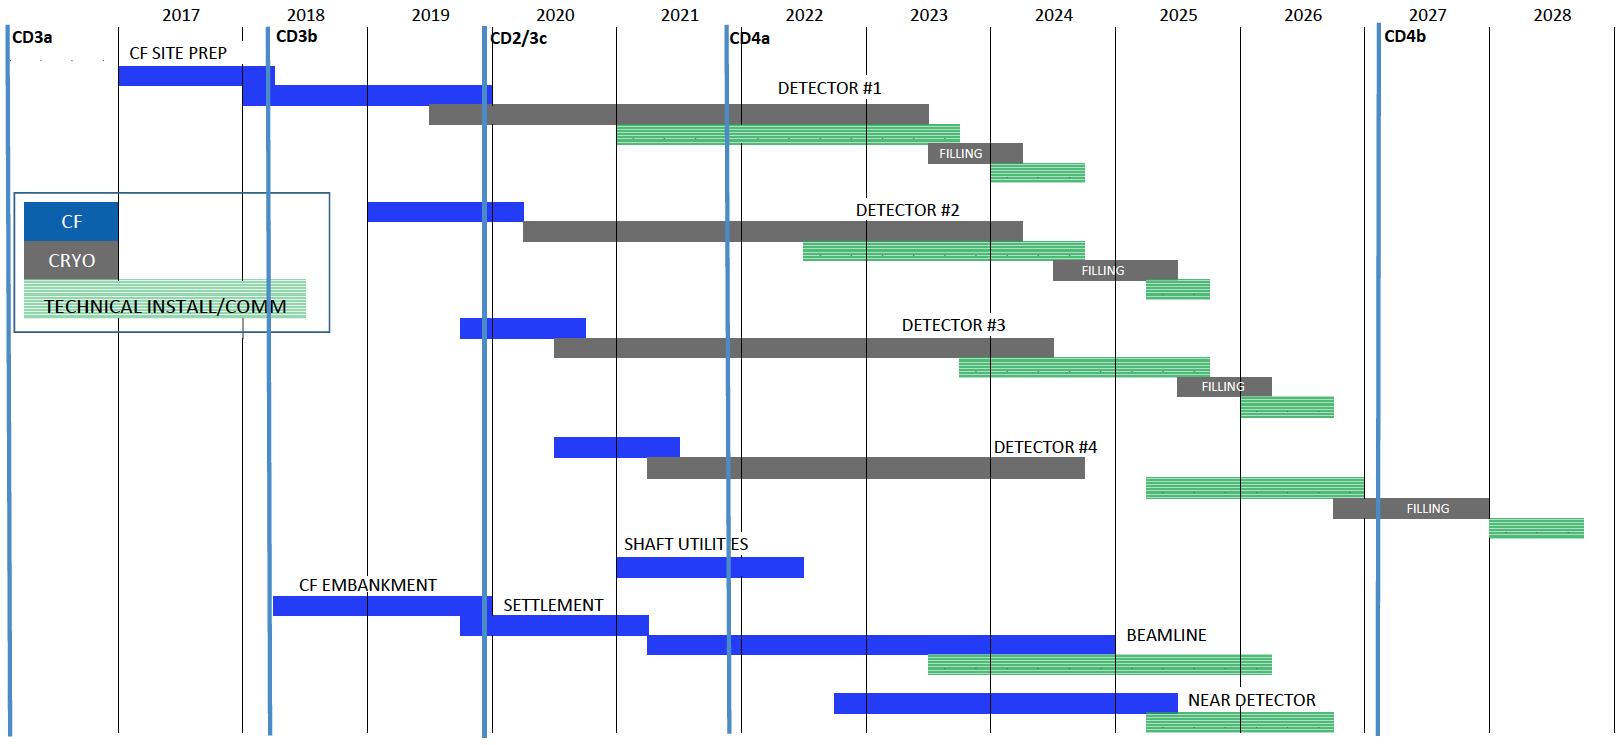
\includegraphics[width=1.2\textwidth, angle=90]{summary-schedule.png}
\end{cdrfigure}


Within the anticipated DOE funding profile, in particular during the initial phase of the project, the far site conventional
facilities are advanced first; their final design starts in fall 2015. Early site preparation is timed to be completed 
in time to start excavation when the Ross Shaft rehabilitation work finishes
 in late 2017. As each detector 
 cavern is excavated and sufficient utilities are installed, the cryostat and cryogenics system work proceeds, followed by detector installation, filling and commissioning. 
 The far detector module \#1 is to be operational by 2024 with modules \#2 and \#3 completed
 one and two years later, respectively, and module \#4 completed by early 2027.

The near site work is delayed with respect to the far site due to the anticipated funding profile. The near site CF and beamline work essentially slows to nearly a stop %almost no effort 
until design restarts in late 2017. Optimization decisions about the beamline that affect the CF design will need to be made by late 2018 in order to be ready for the CF design process. The embankment is constructed and then allowed to settle for at least twelve months before the majority of the beamline CF work proceeds. The beneficial occupancies of the various beamline facilities %CF 
are staggered to allow beamline installation to begin as soon as possible. With this timescale, the far detector science program % with the Far Detectors 
starts with the first module installed and no beam, focusing on non-accelerator-based science %, since 
for slightly more than one year until 
the beamline installation is completed.


The near detector CF construction overlaps that for the beamline, but lags due to available funding. The near detector assembly begins on the surface before beneficial occupancy, after which the detector is installed, complete at about the same time as far detector module \#4. 

The DOE project management process requires approvals at Critical Decision milestones, which allow the LBNF/DUNE project to move to the next step. In fall 2015 the far site CF will seek CD-3a approval for construction of some of the CF and cryogenics systems at SURF. In spring 2018 LBNF near site CF will seek CD-3b construction approval for Advanced Site Preparation to build the embankment. In 2020 LBNF and DUNE will seek to baseline the LBNF/DUNE scope of work, cost and schedule, as well as construction approval for the balance of the project scope of work. 
%% MAT - feel current version is fine \fixme{SP question about balance of scope and is it just about construction approval. I.e., should it read: ``LBNF and DUNE will seek to baseline the LBNF/DUNE scope of work, cost, schedule and construction approval for the balance of the Project scope of work.''?}
The project concludes with CD-4 approval to start operations.

